\documentclass[handout]{beamer}

\usetheme[progressbar=frametitle]{metropolis}
\metroset{block=fill}

\subtitle{NTIN071 Automata and Grammars}
\author{Jakub Bulín (KTIML MFF UK)}

\date{Spring 2025\\ 
    \vspace{1in} 
    \begin{flushleft}
        \it \footnotesize * Adapted from the Czech-lecture slides by Marta Vomlelová with gratitude. The translation, some modifications, and all errors are mine.
    \end{flushleft}
}

%% packages

\usepackage{amsmath}
\usepackage{amssymb}
\usepackage{amsthm}
\usepackage{cancel}
\usepackage{color}
\usepackage{colortbl}
\usepackage{forest}
\usepackage[utf8x]{inputenc}
\usepackage{multicol}
\usepackage{multirow}

%% colors
\definecolor{Gray}{gray}{0.9}

%% TikZ
\usepackage{tikz}
    \usetikzlibrary{
        automata,
        arrows,
        backgrounds,
        decorations.pathmorphing,
        fit,
        positioning,
        shapes,
        shapes.geometric,
        tikzmark
    } 
    \tikzset{>=stealth',shorten >=1pt,auto,node distance=2cm}
    \tikzset{initial text={}}
    \tikzset{elliptic state/.style={draw,ellipse}}

%% amsthm
\theoremstyle{plain}
    \newtheorem*{algorithm}{Algorithm}    
    \newtheorem*{observation}{Observation}
    \newtheorem*{proposition}{Proposition}

\theoremstyle{remark}
    \newtheorem*{exercise}{Exercise}
    \newtheorem*{remark}{Remark}

%% macros
\DeclareMathOperator{\RegE}{RegE}
\DeclareMathOperator{\RL}{RL}

% Just for Lecture 2
\newcommand{\x}{$\times$}
\newcommand{\nx}{\ }



\title{Lecture 7 -- The CYK algorithm, Pushdown automata}


\begin{document}


\frame{\titlepage}


\begin{frame}{Recap of Lecture 6}
	
    \begin{itemize}
		\item Reducing a grammar: removing $\epsilon$-productions, unit productions, useless symbols
		\item Chomsky Normal Form of a context-free grammar
		\item Pumping lemma for context-free languages, application: proving non-context-freeness		
	\end{itemize}
	
\end{frame}


\section{2.8 The CYK algorithm}


\begin{frame}{Testing membership in a context-free language}

	Given a context-free grammar $G$ \alert{in Chomsky Normal Form} and a word $w=a_1\dots a_n\in T^*$, determine if $w\in L(G)$.

	\bigskip

	\textbf{Naive, inefficient algorithm:}
	
	Construct all parse trees from $G$ of appropriate depth ($\lceil log_2|w|\rceil$), check if the yield is $w$.

	\bigskip


	\textbf{The Cocke-Younger-Kasami algorithm:} 
	
	Use \alert{dynamic programming} to compute, for every $1\leq i\leq j\leq n$, the set $X_{ij}$ of all variables of $G$ that generate the subword $a_i\dots a_j$.

	Then check if $S\in X_{1n}$.

	(Very efficient, worst-case time complexity $\mathcal O(n^3|G|)$.)

\end{frame}


\begin{frame}{The CYK algorithm}

	\begin{itemize}
		\item \textbf{input:} $G=(V,T,\mathcal P,S)$ in ChNF, $w=a_1\dots a_n\in T^*$
		\item \textbf{decide:} $w\in L(G)$?
	\end{itemize}	
	
	\begin{multicols}{2}
		Compute for $1\leq i\leq j\leq n$:
		
		\vspace{-24pt}
		$$
		X_{ij}=\{A\in V\mid A\Rightarrow^* a_ia_{i+1}\ldots a_j\}
		$$
		\vspace{-24pt}

		using dynamic programming (storing results in a table)
		
		\begin{center}
			\scalebox{0.85}{
				\begin{tabular}{|c c c c c c c c}
					$X_{15}$ \\ 		
					$X_{14}$ &  $X_{25}$  \\ 
					$X_{13}$ &  $X_{24}$ &  $X_{35}$ \\
					$X_{12}$ &  $X_{23}$ & $X_{34}$ &  $X_{45}$ \\ 
					$X_{11}$ & $X_{22}$ &  $X_{33}$ &$X_{44}$ &$X_{55}$ \\ \hline
					\rowcolor{Gray}$a_1$&$a_2$&$a_3$&$a_4$&$a_5$
				\end{tabular}
			}		
		\end{center}		
	\end{multicols}

	\begin{enumerate}
		\item \textbf{Initialize:} $X_{ii}=\{A\in V\mid A\to a_i \in \mathcal P\}$
		\item \textbf{Fill upwards:} $$X_{ij}=\{A\in V\mid A\to BC\in \mathcal P,B\in X_{ik}, C\in X_{k+1,j}\}$$
		\item \textbf{Check:} Is $S\in X_{1n}$?
	\end{enumerate}	

\end{frame}


\begin{frame}{The CYK algorithm: an example}

	\begin{example}
	$G=(\{S,A,B,C\},\{a,b\},\mathcal P,S)$ with $\mathcal P=\{S\to AB\mid BC, A\to BA\mid a, B\to CC\mid b, C\to AB\mid a\}$
	\end{example}
	\vspace{-6pt}
	Rules reversed:\vspace{-6pt}
	\begin{quote}
		\begin{multicols}{4}\small
			$AB  \leftarrow  \{S,C\}$\\
			$BA  \leftarrow  \{A\}$\\
			$BC  \leftarrow  \{S\}$\\
			$CC  \leftarrow  \{B\}$\\
			$b   \leftarrow  \{B\}$\\
			$a   \leftarrow  \{A,C\}$
		\end{multicols}	
	\end{quote}

	\vspace{-12pt}
	Fill upwards:
	\vspace{3pt}

	\begin{center}
		\begin{tabular}{|c c c c c c c c}
			$\{\alert{S},A,C\}$ \\ 
			- &  $\{S,A,C\}$  \\ 
			- &  $\{B\}$ &  $\{B\}$ \\ 
			$\{S,A\}$ &  $\{B\}$ & $\{S,C\}$ &  $\{S,A\}$ \\ 
			$\{B\}$ & $\{A,C\}$ &  $\{A,C\}$ &$\{B\}$ &$\{A,C\}$ \\ %\cline{1-7}
			\rowcolor{Gray}$b$&$a$&$a$&$b$&$a$
		\end{tabular}
	\end{center}

\end{frame}


\begin{frame}{Testing emptiness of a context-free language}

    \vspace{-4pt}
    \begin{center}
        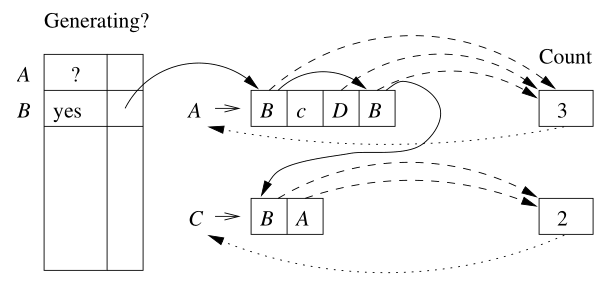
\includegraphics[width=0.8\textwidth]{files/emptyCFL.PNG}    
    \end{center}
    \vspace{-18pt}
    Is the start symbol $S$ generating? Can be done in $O(|G|)$ time. 
    \vspace{-4pt}   
    \begin{itemize}
        \item For each variable a chain of all body positions where it appears
        \item For each production two-way link to a count of body positions with variables that have not yet been marked as generating
    \end{itemize}
    \vspace{-4pt}
    Once we mark a variable as generating, follow the chain and decrease counts by $1$. If a count reaches $0$, mark the head as generating. Process all generating variables using a stack.
    
\end{frame}


\begin{frame}{Testing finiteness of a context-free language}

    Let $G$ be a Chomsky normal form grammar for $L$, i.e. $L\setminus\{\lambda\}=L(G)$. Construct the following oriented graph: 
    \begin{itemize}
        \item nodes: variables in $G$
        \item edges: $\{(A,B),(A,C) \mid A\rightarrow BC\text{ is a production rule in }G\}$
    \end{itemize}
    Now $L$ is infinite, if and only if the graph contains an oriented cycle. Can be tested in $O(|G|)$.


\end{frame}


\section{2.9 Pushdown automata}


\begin{frame}{Pushdown automaton (PDA)}

    \vspace{-6pt}
    \begin{center}
        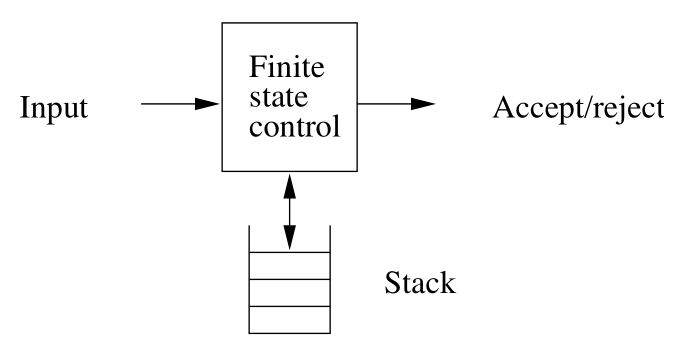
\includegraphics[width=0.6\textwidth]{files/pushDown.PNG}
    \end{center}
    \vspace{-12pt}

    \begin{itemize}
        \item an extension of $\epsilon$--NFA, additional feature: a \alert{stack} memory %(push, pop -- only at the top)
        \item the stack has its own \alert{stack alphabet} $\Gamma$ (can contain $\Sigma$ or not)
        \item at each step we pop the top stack symbol $X$, make a decision based on $(q,a,X)$, push some word $\gamma\in\gamma^*$
        \item the stack can rememeber an infinite amount of information
        \item PDA define context-free languages, nondeterminism is important: \alert{deterministic} PDA only recognize a proper subset of context-free languages (unlike DFA vs. NFA)
    \end{itemize}
    
\end{frame}


\begin{frame}{The definition}

    \alert{A pushdown automaton} (\alert{PDA}): $P=(Q,\Sigma,\Gamma,\delta,q_0,Z_0,F)$, where
        
    \begin{itemize}
        \item $Q$ is finite, nonempty set of states
        \item $\Sigma$ is a finite, nonempty \alert{input alphabet}
        \item $\Gamma$ is a finite, nonempty \alert{stack alphabet}
        \item $\delta$ is the \alert{transition function}, 
        $$
        \delta\colon Q\times (\Sigma\cup \{\epsilon\})\times \Gamma \to \mathcal P_{FIN}(Q \times \Gamma^*)
        $$ 
        $\delta(q,a,X)\ni(p,\gamma)$ where $p$ is the new state and $\gamma$ a finite string of stack symbols that \alert{replace} $X$ on top of the stack
        \item $q_0\in Q$ is the \alert{initial state}
        \item $Z_0\in\Gamma$ is the \alert{initial stack symbol} (\alert{bottom of the stack}); the only symbol on the stack at the beginning
        \item $F$ is a set of \alert{accepting} (\alert{final}) states; may be undefined if our PDA \alert{accepts by empty stack}
    \end{itemize}

\end{frame}


\begin{frame}{One transition of a PDA}   

    \begin{itemize}
        \item read one input letter ($a\in\Sigma$) or do an $\epsilon$-transition ($a=\epsilon$)
        \item pop $X$ from the top of the stack
        \item based on $a$, $X$, and the current state $q$ nondeterministically choose one of finitely many options $(p,\gamma)\in\delta(q,a,X)$
        \item switch to the new state $p$
        \item push the finite string $\gamma$ to the stack (the first symbol of $\Gamma$ is now on top)
        \item \alert{pop}: $\gamma=\epsilon$, \alert{read} only: $\gamma=X$, \alert{push}: $\gamma=\gamma'X$
\end{itemize}

\end{frame}


\begin{frame}{Example: $L_{wwr}=\{ww^R\mid w \in \{0,1\}^*\}$}

    \begin{center}
        \scalebox{0.95}{
        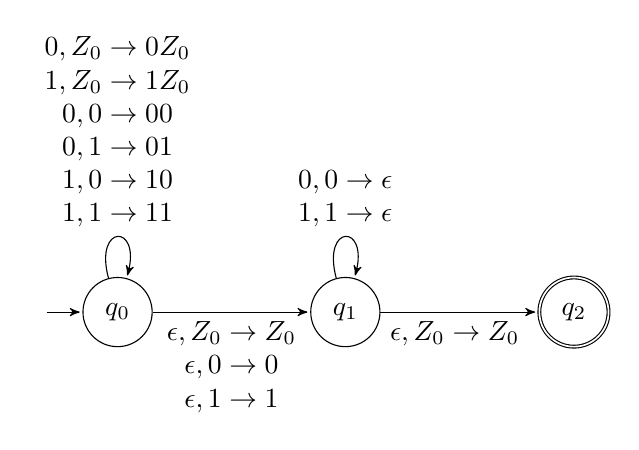
\begin{tikzpicture}[]
            \node[initial,state] (q0)      {$q_0$};
            \node[state] (q1)  [right=2cm of q0]     {$q_1$};
            \node[state, accepting] (q2)  [right=2cm of q1]    {$q_2$};
            \path[->]
                (q0)  edge[loop above]  node[align=center] {
                                        $0,Z_0 \rightarrow 0Z_0$	\\
                                        $1,Z_0 \rightarrow 1Z_0$	\\			
                                        $0,0 \rightarrow 00$	\\			
                                        $0,1 \rightarrow 01$	\\			
                                        $1,0 \rightarrow 10$	\\			
                                        $1,1 \rightarrow 11$			
                                        } (q0)
                (q0)  edge[swap]  node[align=center] {
                                        $\epsilon,Z_0 \rightarrow Z_0$	\\			
                                        $\epsilon,0 \rightarrow 0$	\\			
                                        $\epsilon,1 \rightarrow 1$			
                                        }  (q1)
                (q1)  edge[loop above]  node[align=center] {
                                        $0,0 \rightarrow \epsilon$	\\			
                                        $1,1 \rightarrow \epsilon$			
                                        } (q1)
                (q1)  edge[swap]  node[align=center] {
                                        $\epsilon,Z_0 \rightarrow Z_0$	
                                        } (q2)
                ;
        \end{tikzpicture}
        }
    \end{center}

    \vspace{-12pt}   
    
    \alert{$q_0$} read input letters pushing them onto the stack; guess the middle (nondeterministically), jump to $q_1$\\
    \alert{$q_1$} compare input with stack, consuming both; if empty stack (we see the bottom), accept by jumping to $q_2$; no input can remain

\end{frame}


\begin{frame}{Example cont'd: full description of the PDA}

    \begin{center}
        $P=(\{q_0,q_1,q_2\},\{0,1\},\{0,1,Z_0\},\delta,q_0,Z_0,\{q_2\})$
    \end{center}

    \begin{tabular}{l l}\hline
        $\delta(q_0,0,Z_0)=\{(q_0,0Z_0)\}$ &  
            \multirow{2}{*}{push input onto stack, leave the bottom} \\
        $\delta(q_0,1,Z_0)=\{(q_0,1Z_0)\}$ &  \\\hline
        $\delta(q_0,0,0)=\{(q_0,00)\}$ &  
            \multirow{4}{*}{stay in $q_0$, push input onto stack}\\ 
        $\delta(q_0,0,1)=\{(q_0,01)\}$ \\
        $\delta(q_0,1,0)=\{(q_0,10)\}$ \\
        $\delta(q_0,1,1)=\{(q_0,11)\}$ \\ \hline
        $\delta(q_0,\epsilon,Z_0)=\{(q_1,Z_0)\}$ &
            \multirow{3}{*}{jump to $q_1$ without changing stack}\\ 
        $\delta(q_0,\epsilon,0)=\{(q_1,0)\}$ \\
        $\delta(q_0,\epsilon,1)=\{(q_1,1)\}$ \\ \hline
        $\delta(q_1,0,0)=\{(q_1,\epsilon)\}$ &
            \multirow{2}{*}{pop stack and match with input}\\ 
        $\delta(q_1,1,1)=\{(q_1,\epsilon)\}$ \\ \hline
        $\delta(q_1,\epsilon,Z_0)=\{(q_2,Z_0)\}$ & we have $ww^R$, go to accepting state
        \\\hline
    \end{tabular}

\end{frame}


\begin{frame}{Notation}

    \begin{center}
        \begin{tabular}{l l}
            $a,b,c$ & symbols of the input alphabet\\
            $q,p, r$ & states\\
            $u,w,x,y,z$ & words over input alphabet\\
            $X,Y,A,B$ & stack symbols\\
            $Z_0$ & bottom of the stack symbol\\
            $\alpha,\beta,\gamma$ & words over stack alphabet		
        \end{tabular}
    \end{center}

    \bigskip

    Transition diagram:
    \begin{itemize}
        \item nodes are states, initial and final denoted as usual
        \item a transition $\delta(q,a,X)\ni (p,\alpha)$: arc from $p$ to $q$ labelled $a,X\rightarrow \alpha$          
    \end{itemize}

\end{frame}


\section*{The languages of a PDA}


\begin{frame}{Configurations and moves (computation graph)}

    A \alert{configuration} of a PDA is a triple \alert{$(q,w,\gamma)$}, where
    \begin{description}
        \item[$q$] is the current state 
        \item[$w$] is the remaining input and
        \item[$\gamma$] is the stack contents (the top is on the left) 
    \end{description}

    We define \alert{moves} between configurations (\alert{$\vdash_P$} or \alert{$\vdash$}) thus: for any transition $\delta(q,a,X)\ni(p,\alpha)$ and all $w\in \Sigma^*$ and $\beta\in \Gamma^*$ we have
    $$
    (q,aw,X\beta)\vdash (p,w,\alpha\beta)
    $$
    We use the symbol \alert{$\vdash^*_P$} or \alert{$\vdash^*$} to represent zero or more moves, i.e.
    \begin{itemize}
        \item $I\vdash^*I$ for any configuration $I$
        \item $I\vdash^*J$ if there exists $K$ such that $I\vdash K$ and $K\vdash^*J$
    \end{itemize}

\end{frame}


\begin{frame}{Initial and accepting configurations, the languages of a PDA}

    The \alert{initial configuration} of $P=(Q,\Sigma,\Gamma,\delta,q_0,Z_0,F)$ for input word $w\in\Sigma^*$ is \alert{$(q_0,w,Z_0)$}. Which configurations are \alert{accepting}? 
    
    Two options:

    \textbf{1. Acceptance by final state:} \alert{$(f,\epsilon,\gamma)$} for some final state $f\in F$ and arbitrary stack contents $\gamma\in\Gamma^*$


    $\alert{L(P)}=\{w\mid (q_0,w,Z_0)\vdash^*_P (f,\epsilon,\gamma)\text{ for some }f\in F\text{ and }\gamma\in\Gamma^*\}$

    \bigskip

    \textbf{2. Acceptance by empty stack:} \alert{$(q,\epsilon,\epsilon)$} for an arbitrary $q\in Q$

    $\alert{N(P)}=\{w\mid (q_0,w,Z_0)\vdash^*_P (q,\epsilon,\epsilon)\text{ for any }q\in Q\}$

    \medskip

    In this case we can write only $P=(Q,\Sigma,\Gamma,\delta,q_0,Z_0)$    

\end{frame}


\begin{frame}{Configurations for the input $w=1111$}

    \begin{center}
        \scalebox{0.8}{
            \begin{forest}
                for tree={edge=->}
                [{$(q_0, 1111, Z_0)$},tikz={\node [draw,green,fit=()] {};}
                    [{$(q_0, 111, 1Z_0)$}
                    [{$(q_0, 11, 11Z_0)$}
                    [{$(q_0, 1, 111Z_0)$}
                    [{$(q_0, \epsilon, 1111Z_0)$}[{$(q_1, \epsilon, 1111Z_0)$}]]
                    [{$(q_1, 1, 111Z_0)$}[{$(q_1, \epsilon, 11Z_0)$}]]]
                    [{$(q_1, 11, 11Z_0)$}[{$(q_1, 1, 1Z_0)$}[{$(q_1, \epsilon, Z_0)$}[{$(q_2, \epsilon, Z_0)$},tikz={\node [draw,red,fit=()] {};}]]]]
                    ]
                [{$(q_1, 111, 1Z_0)$}[{$(q_1, 11, Z_0)$}[{$(q_2, 11, Z_0)$}]]]
                ]
                [{$(q_1, 1111, Z_0)$}[{$(q_2, 1111, Z_0)$}]]
                ]
            \end{forest}
        }
    \end{center}

\end{frame}


\begin{frame}{Our example}

    \begin{center}
        \scalebox{0.85}{
        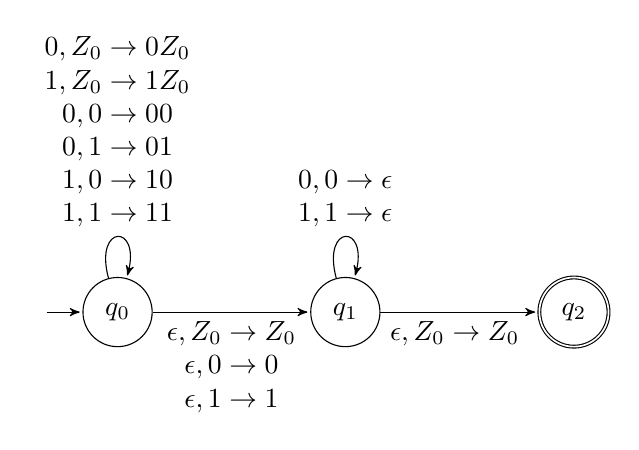
\begin{tikzpicture}[]
            \node[initial,state] (q0)      {$q_0$};
            \node[state] (q1)  [right=2cm of q0]     {$q_1$};
            \node[state, accepting] (q2)  [right=2cm of q1]    {$q_2$};
            \path[->]
                (q0)  edge[loop above]  node[align=center] {
                                        $0,Z_0 \rightarrow 0Z_0$	\\
                                        $1,Z_0 \rightarrow 1Z_0$	\\			
                                        $0,0 \rightarrow 00$	\\			
                                        $0,1 \rightarrow 01$	\\			
                                        $1,0 \rightarrow 10$	\\			
                                        $1,1 \rightarrow 11$			
                                        } (q0)
                (q0)  edge[swap]  node[align=center] {
                                        $\epsilon,Z_0 \rightarrow Z_0$	\\			
                                        $\epsilon,0 \rightarrow 0$	\\			
                                        $\epsilon,1 \rightarrow 1$			
                                        }  (q1)
                (q1)  edge[loop above]  node[align=center] {
                                        $0,0 \rightarrow \epsilon$	\\			
                                        $1,1 \rightarrow \epsilon$			
                                        } (q1)
                (q1)  edge[swap]  node[align=center] {
                                        $\epsilon,Z_0 \rightarrow \alert{Z_0}$	
                                        } (q2)
                ;
        \end{tikzpicture}
        }
    \end{center}

    \begin{itemize}
        \item acceptance by final state: $L(P)=L_{wwr}$
        \item to accept by empty stack: modify $\delta(q_1,\epsilon,Z_0)=\{(q_2,Z_0)\}$ to $\delta(q_1,\epsilon,Z_0)=\{(q_2,\epsilon)\}$ (erase bottom of the stack symbol), then also $N(P')=L_{wwr}$
    \end{itemize}

\end{frame}


\begin{frame}{Another example: if-else}

    Stop (accept) at first error, e.g. more $\mathtt{else}$'s than $\mathtt{if}$'s

    \textbf{By empty stack:} {\small $P_N=(\{q\},\{\mathtt{if},\mathtt{else}\},\{Z\},\delta_N,q,Z)$}

    \begin{columns}

        \small

        \column{0.48\textwidth}

        \begin{center}
            \scalebox{0.87}{
                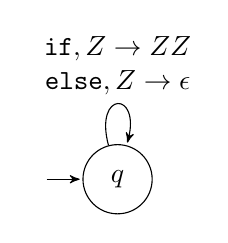
\begin{tikzpicture}
                    \node[initial,state] (q) {$q$};
                    \path[->]
                        (q)  edge[loop above] node[align=center] { $\mathtt{if},Z\rightarrow ZZ$\\ $\mathtt{else},Z\rightarrow \epsilon$} (q);
                \end{tikzpicture}
            }
        \end{center} 

        \column{0.52\textwidth}

        \begin{itemize}
            \item[] $\delta_N(q,\mathtt{if},Z)=\{(q,ZZ)\}$ \hfill(push)
            \item[] $\delta_N(q,\mathtt{else},Z)=\{(q,\epsilon)\}$ \hfill(pop)
        \end{itemize}
        
    \end{columns}

    \medskip

    \textbf{By final state:} {\small $P_F=(\{p,q,r\},\{\mathtt{if},\mathtt{else}\},\{Z,X_0\},\delta_F,p,X_0,\{r\})$}

    \begin{columns}

        \small

        \column{0.48\textwidth}

        \begin{center}
            \scalebox{0.87}{
                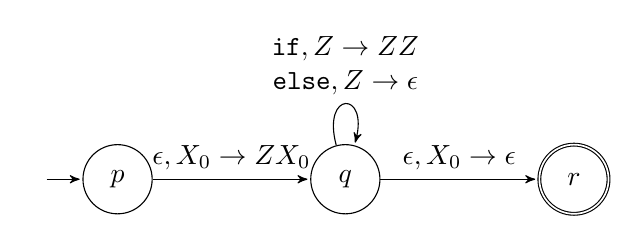
\begin{tikzpicture}
                    \node[initial,state] (p)      {$p$};
                    \node[state] (q) [right=2cm of p]     {$q$};
                    \node[state,accepting] (r) [right=2cm  of q]     {$r$};
                    \path[->]
                        (q)  edge[loop above] node[align=center] { $\mathtt{if},Z\rightarrow ZZ$\\ $\mathtt{else},Z\rightarrow \epsilon$} (q)
                        (p)  edge node {$\epsilon,X_0\rightarrow ZX_0$} (q)
                        (q)  edge node {$\epsilon,X_0\rightarrow \epsilon$} (r);
                \end{tikzpicture}
            }
        \end{center}          
        
        \column{0.52\textwidth}
        
        \begin{itemize}
            \item[] $\delta_F(p,\epsilon,X_0)=\{(q,ZX_0)\}$ \hfill (start)
            \item[] $\delta_F(q,\mathtt{if},Z)=\{(q,ZZ)\}$ \hfill (push)
            \item[] $\delta_F(q,\mathtt{else},Z)=\{(q,\epsilon)\}$ \hfill (pop)
            \item[] $\delta_F(q,\epsilon,X_0)=\{(r,\epsilon)\}$ \hfill (accept)
        \end{itemize}
        
    \end{columns}

\end{frame}


\begin{frame}{From empty stack to final state}

    \begin{lemma}
        If $L=N(P_N)$ for some PDA $P_N=(Q,\Sigma,\Gamma,\delta_N,q_0,Z_0)$, then there is a PDA $P_F$ such that $L=L(P_F)$.
    \end{lemma}

    \begin{center}
        \scalebox{0.9}{
            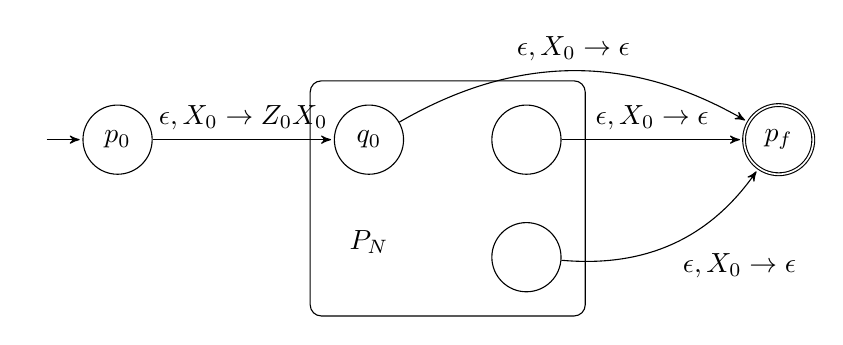
\begin{tikzpicture}
                \node[initial,state] (p0)      {$p_0$};
                \node[state] (q0)  [right=2.3cm of p0]    {$q_0$};
                \node[state] (q1a)   [right of=q0]   {};
                \node[state] (q1b)   [below=.6cm of q1a]   {};
                \node[state,draw=none] (pf) [below=.4cm of q0] {$P_N$};
                \node[state,accepting] (q2)   [right=2.3cm of q1a] {$p_f$};
                \node[state] (X)[rectangle,  fit= (q0) (q1a) (q1b), inner sep=0.3cm,rounded corners] {};
                \path[->]
                    (p0)  edge node {$\epsilon,X_0 \rightarrow Z_0X_0$} (q0)
                    (q0)  edge[bend left] node {$\epsilon, X_0\rightarrow \epsilon$} (q2)
                    (q1a)  edge node {$\epsilon, X_0\rightarrow \epsilon$} (q2)
                    (q1b)  edge[bend right] node[swap] {$\epsilon,X_0\rightarrow \epsilon$} (q2);        
            \end{tikzpicture}
        }
    \end{center}

    \textbf{Idea:} Make $Z_0$ a fake bottom (insert a new bottom $X_0$ below), so that we can tell when $P_N$'s stack was empty. Add $\epsilon$-transitions upon seeing $X_0$ from all states to a new, accepting state.

\end{frame}


\begin{frame}{The proof}

    $P_F=(Q\cup \{p_0,p_f\},\Sigma,\Gamma\cup\{X_0\},\delta_F,p_0,X_0,\{p_F\})$, where $\delta_F$ is
    \begin{itemize}
        \item $\delta_F(p_0,\epsilon,X_0)=\{(q_0,Z_0X_0)\}$ (start).
        \item $\forall (q\in Q, a\in \Sigma\cup\{\epsilon\},Y\in \Gamma)$, $\delta_F(q,a,Y)=\delta_N(q,a,Y)$.
        \item In addition, $\delta_F(q,\epsilon,X_0)\ni (p_f,\epsilon)$ for every $q\in Q$.
    \end{itemize}
    We must show that $w\in L(P_N)$ iff $w\in L(P_F)$.
    \begin{itemize}
        \item (If) $P_F$ accepts as follows: $(p_0,w,X_0)\vdash_{P_F}(q_0,w,Z_0X_0)\vdash^*_{P_F=N_F}(q,\epsilon,X_0)\vdash_{P_F}(p_f,\epsilon,\epsilon) $.
        \item (Only if) No other way to go to $p_F$ than the above. \hfill\qedsymbol
    \end{itemize}
    

\end{frame}


\begin{frame}{From final state to empty stack}

    \begin{lemma}
        If $L=L(P_F)$ for some PDA  
        $P_F=(Q,\Sigma,\Gamma,\delta_F,q_0,Z_0,F)$, then there exists a PDA $P_N$ such that $L=N(P_N)$.
    \end{lemma} 
    
    \begin{center}
        \scalebox{0.95}{
            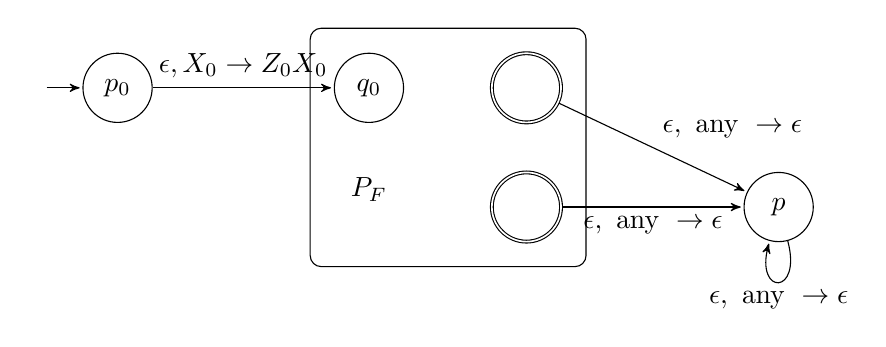
\begin{tikzpicture}
                \node[initial,state] (p0)      {$p_0$};
                \node[state] (q0)  [right=2.3cm of p0]    {$q_0$};
                \node[state,accepting] (q1a)   [right of=q0]   {};
                \node[state,accepting] (q1b)   [below=.6cm of q1a]  {};
                \node[state,draw=none] (pf) [below=.4cm of q0] {$P_F$};
                \node[state] (q2)   [right=2.3cm of q1b] {$p$};
                \node[state] (X)[rectangle,  fit= (q0) (q1a) (q1b), inner sep=0.3cm,rounded corners] {};
                \path[->]
                    (p0)  edge node {$\epsilon,X_0 \rightarrow Z_0X_0$} (q0)
                    (q1a)  edge node {$\epsilon, \hbox{ any }\rightarrow \epsilon$} (q2)
                    (q1b)  edge node[swap] {$\epsilon,\hbox{ any }\rightarrow \epsilon$} (q2)
                    (q2)  edge[loop below] node {$\epsilon,\hbox{ any }\rightarrow\epsilon$} (q2);
            \end{tikzpicture}            
        }
    \end{center}
    \vspace{-12pt}

    \textbf{Idea:} Make $Z_0$ a fake bottom (insert a new bottom below), because $P_F$ could accidentally empty stack in a nonfinal state. Add $\epsilon$-transitions (upon any stack symbol) from final states to a new state, there empty the stack without reading any input symbols.

\end{frame}


\begin{frame}{The proof}

    Let $P_N=(Q\cup \{p_0,p\},\Sigma,\Gamma\cup\{X_0\},\delta_N,p_0,X_0)$, where
    \begin{itemize}
        \item $\delta_N(p_0,\epsilon,X_0)=\{(q,Z_0X_0)\}$ (start)
        \item $\forall (q\in Q, a \in \Sigma\cup\{\epsilon\},Y\in \Gamma)$ $\delta_N(q,a,Y)=\delta_F(q,a,Y)$ (simulate)
        \item $\forall (q \in F,Y\in \Gamma\cup\{X_0\})$, $\delta_N(q,\epsilon,Y)\ni (p,\epsilon)$ (i.e. accept if $P_F$ accepts)
        \item $\forall (Y\in \Gamma\cup\{X_0\}), \delta_N(p,\epsilon,Y)=\{ (p,\epsilon)\}$ clean the stack.
    \end{itemize}
    The proof $w\in N(P_N)$ iff $w\in L(P_F)$ is similar as before.\hfill\qedsymbol

\end{frame}


\begin{frame}{Unseen data cannot affect computation}

    \begin{lemma}
        If $(q,x,\alpha)\vdash_P (p,y,\beta) $, then for any $w\in \Sigma^*$ and $\gamma\in\Gamma^*$ we also have 
        $(q,xw,\alpha\gamma)\vdash^*_P(p,yw,\beta\gamma)$. (In particular, $\gamma=\epsilon$ or $w=\epsilon$.)
    \end{lemma}
    \textbf{Proof:} Induction on the number length of the sequence of configurations that take $(q,xw,\alpha\gamma)$ to $(p,yw,\beta\gamma)$. Each of the moves $(q,x,\alpha)\vdash^*_P(p,y,\beta)$ is justified without using $w$ and/or $\gamma$ in any way. The moves are still valid with $w,\gamma$ on the input/stack.\hfill\qedsymbol

    \medskip

    \begin{lemma}
        If $(q,xw,\alpha)\vdash^*_P (p,yw,\beta) $, then also $(q,x,\alpha)\vdash^*_P(p,y,\beta)$.
    \end{lemma}
    \textbf{NB:} Not true for stack, the computation may require $\gamma$ on the stack and then push it back. (E.g. $L=\{0^i1^i0^j1^j\}$, configuration $(p,0^{i-j}1^i0^j1^j,0^jZ_0)\vdash^* (q,1^j,0^jZ_0)$, inbetween clear the stack.)

\end{frame}


\begin{frame}{Summary of Lecture 7}
	
	\begin{itemize}    
        \item Testing membership in a context-free language: the Cocke-Younger-Kasami algorithm
        \item Testing emptiness and finiteness of a context-free language    
		\item Pushdown automaton: extend an $\epsilon$-NFA with a stack memory (potentially infinite), pop the top symbol, decide based on $(q,a,X)$, can push a finite string of stack symbols
        \item Acceptance by final state $L(P)$ and by empty stack $N(P)$, conversion between the two options        	
	\end{itemize}

\end{frame}


\end{document}
